\documentclass[12pt]{article}

\usepackage{cite}
\usepackage{graphicx}
\usepackage[margin=1in]{geometry}
\usepackage[font=small,labelfont=bf]{caption}

\begin{document}

\begin{center}
	\Large
    	\textbf{Spiral Packing - Milestone II Evaluation}
    
    	\vspace{0.1cm}
    	\large
    	\textbf{Adrian Cortez}
	
	\vspace{0.1cm}	
	\small
    	\textbf{Advisor: Dr. Roger Gaborski}
        
    	\vspace{0.1cm}
    	\small
    	\textbf{Rochester Institute of Technology}
    	\vspace{0.3cm}
\end{center}

	The primary goal for Milestone II -- and what was identified as the first task to work on after Milestone I -- was to implement the fitting algorithm as described in the paper ``Spiral Packing'' by Cameron Browne and Paul van Wamelen \cite{Browne2006834} for the three general branching cases shown in Figure~\ref{fig:geo}. The algorithm proposed in the paper is an iterative algorithm, meaning it will eventually converge on an acceptable placement for a child spiral after a number of iterations. At each iteration, a better estimation is made for the determined child position and orientation based on the new state of the packed area. The algorithm returns when the child spiral no longer intersects any non-parent spirals and the child spiral is deemed a good fit if its position is close to the original user-specified position.\cite{Browne2006834} Along with the implementation, several images generated using the implemented algorithm were delivered to demonstrate the primary results of the program. The secondary goal for this milestone was to draft the introduction and background sections of the final paper.
	
\begin{figure}[ht]
	\centering
	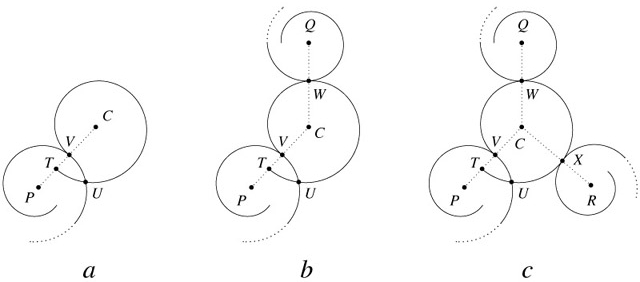
\includegraphics[width=90mm,height=40mm]{spiral-packing-fig-01}
	\caption{The three geometric cases when branching: (a) simple branching, (b) fitting the child spiral to one neighboring spiral, and (c) fitting the child spiral to two neighboring spirals. \cite{Browne2006834}}
	\label{fig:geo}
\end{figure}

	To simplify the process of fitting spirals tangent to each other, Browne and Wamelen's algorithm approximates the spirals as circles, updating these approximations at each iteration based on the change in the position and orientation of the child spiral from the previous iteration. Essentially this reduces the spiral packing problem to the circle packing problem, also known as Apollonian packing.\cite{Kasner1943} Figure~\ref{fig:circle} shows an example of circle packing with three tangent circles and demonstrates how circle packing is similar to spiral packing. The circle packing problem is significantly easier to solve mathematically than the numerical solution to the spiral packing problem.\cite{Browne2006834, Kasner1943}

	In addition to solving the circle fitting problem, the spiral fitting algorithm required several supporting functions. These functions handled a variety of aspects of the algorithm, such as detecting when spirals intersected, determining the part of the spirals to clip, and handling user input.
	
\begin{figure}[ht]
	\centering
	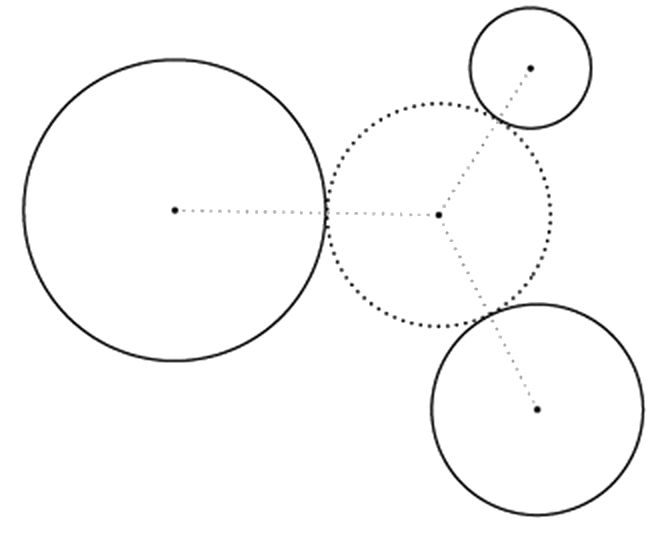
\includegraphics[width=37mm,height=30mm]{spiral-circles}
	\caption{Apollonian Packing. Fitting a circle tangent to three other circles. \cite{Browne2006834}}
	\label{fig:circle}
\end{figure}

	There were two problems encountered when implementing the algorithm for Milestone II. The first problem was that it took slightly longer to work through the math and implement the functions for solving the system of equations that described the circle fitting problem for the three branching cases. The second and most time consuming problem was the oversight of an innocuous variable within the pseudocode presented in Browne and Wamelen's paper. The variable, \textit{rso}, is introduced in the pseudocode of the iterative algorithm for solving the three geometric cases when branching. At every iteration, it is used to offset and correct the radii of the circles used to approximate the spirals before solving the appropriate circle fitting case. The variable was introduced but not described within the paper, leaving its exact function up to interpretation. It was clear, however, that this variable was crucial to getting the algorithm to not only converge on a solution, but potential terminate at all. After spending three days testing several potential formulas for calculating this value, I contacted the primary author of the paper, Dr. Cameron Browne, for his input. Unfortunately, his initial response did not help to solve the problem and no further correspondence has been received. After another couple of days spent slightly modifying the algorithm I was able to find a solution. 
	
	Overall, the combination of these problems required approximately a week of the allotted time for this Milestone to solve. As such, the implemented algorithm that was delivered did not properly handle all edge cases by the milestone deadline. In addition, encountering these issues left less time to properly test the implementation and address any flaws. For example, there is an issue with the clipping of the parent and child after branching were slightly more is clipped than desired. Addressing this issue had to be moved to Milestone III because of the time constraint.
	
	The most important task to accomplish next during Milestone III is the implementation of boundary shapes, within which the packing will occur. This will initially include simple geometric shapes, such as rectangles, circles and triangles with more complex shapes being implemented if time permits. The boundary shapes will be implemented as series of spirals, as suggested by Browne and Wamelen.\cite{Browne2006834} The spirals that make up the boundary shapes will have small widths and a large number of turns so that they essentially become points. This will allow the fitting algorithm to also solve the packing along the boundaries. In addition, adding flat and gradient color to the spirals is an important task to complete for the next milestone. To facilitate the rendering of the spiral paths and the gradient color, JavaScript libraries that create the necessary SVG elements are utilized.
		
\begingroup
\renewcommand{\section}[2]{}%
\bibliographystyle{plain}
\bibliography{references}{}
\endgroup

\end{document}